\subsection{Mobile Network Terminology}
\label{sec:mobile_network_terminology}
A number of terminologies will now be defined and described in order to aid 
further understanding of the project.

\subsubsection{Radio Access Technology}
The Radio Access Technology (RAT) refers to the method in which a given device 
connects to the core network. Examples are:
\begin{itemize}
  \item UTRA (UMTS Terrestrial Radio Access), known simply as 3G
  \item GERAN (GSM EDGE Radio Access Network), known simply as 2G
\end{itemize}

The core network routes traffic through various switches. Each RAT will have 
it's own ``dedicated network''. It is possible however to handover from one 
network to another.

Within this project, these will be referred to by the terms ``Start RAT'' and 
``End RAT''. A section of possible RAT combinations are shown below:
\begin{multicols}{3}
  \begin{itemize}
    \item 2G $\Rightarrow$ 2G
    \item 2G $\Rightarrow$ 3G
    \item 2G $\Rightarrow$ 4G
    \item 3G $\Rightarrow$ 2G
    \item 3G $\Rightarrow$ 3G
    \item 3G $\Rightarrow$ 4G
    \item 4G $\Rightarrow$ 2G
    \item 4G $\Rightarrow$ 3G
    \item 4G $\Rightarrow$ 4G
  \end{itemize}
\end{multicols}

The RAT upon the left hand side of the separator is the Start RAT and the RAT 
upon the right hand side of the separator is the End RAT. So for the given 
example:

\begin{quote}
  2G $\Rightarrow$ 3G
\end{quote}

it would read:

\begin{quote}
  ``The given UE had a Start RAT of 2G and an End RAT of 3G''
\end{quote}


\subsubsection{Frequency}
In order to allow multiple UEs to operate upon the same RAT different 
operator frequencies have to be used \citep{cox08}. However to ensure that 
frequencies are efficiently distrusted, frequencies will be reused by following
a ``frequency reuse plan''. 

This prevents situations where by the some frequencies ``come together'', which
ultimately results in co-channel interference \citep{mpirical10}.

Figure \ref{fig:frequencyReuse} highlights a repeat pattern, in this instance 
a four cell repeat pattern. ``The most important fact about cell planning is 
the reuse distance as this determines when it is possible to reuse the same 
frequency'' \citep{mpirical10}.

\begin{figure}[H]
  \centering
    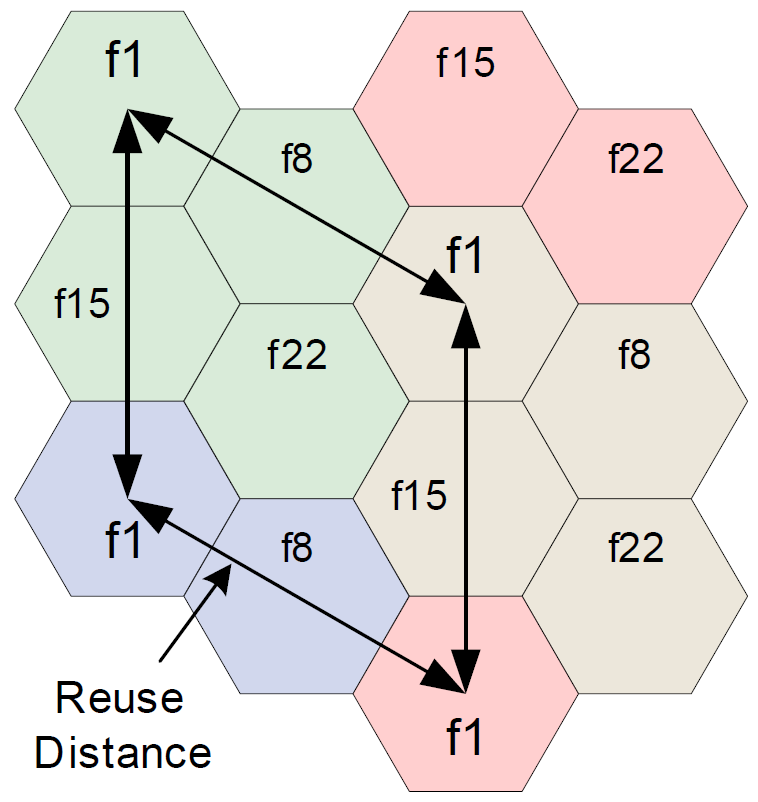
\includegraphics[width=0.4\textwidth]{chapter3/mobile_networks/frequency_reuse.png}
  \caption{An example frequency reuse plan.}.
  \label{fig:frequencyReuse}
\end{figure}

In this example there is always one cell between co-channels, and hence this 
would reduce the interference between the same channels. However it must also 
be mentioned that radio waves do not simply stop at the edge of a cell. 

Signals will ``propagate for many more kilometres'' \citep{mpirical10}. However
because of the reuse distance, the carrier signal --- the wanted signal --- 
should be far more powerful than the interferer signal --- the unwanted signal 
from neighbouring cells --- \citep{mpirical10} .

Within this project the frequency will be referred to as the Mix-Band. This is 
because the Mix-Band refers to 2G, 3G and 4G frequencies and not simply one 
type of frequency. 

Each frequency will comprise of a ``Start Mix-Band'' and an ``End Mix-Band''. 
An example selection of possible Mix-Band combinations are shown below (note 
there could be many hundred):

\begin{multicols}{3}
  \begin{itemize}
    \item GSM 900 $\Rightarrow$ GSM 900
    \item GSM 900 $\Rightarrow$ DCS PCS
    \item GSM 900 $\Rightarrow$ 10763
    \item DCS PCS $\Rightarrow$ GSM 900
    \item DCS PCS $\Rightarrow$ DCS PCS
    \item DCS PCS $\Rightarrow$ 10763
    \item 10763 $\Rightarrow$ GSM 900
    \item 10763 $\Rightarrow$ DCS PCS
    \item 10763 $\Rightarrow$ 10763
  \end{itemize}
\end{multicols}


\subsubsection{Radio Resource Control}
The Radio Resource Control (RRC) is found within layer three (the network 
layer) of the OSI Seven Layer Model. The RRC is the routing manager, and will 
contain various routing options that are stored in a routing table. 
The routing table is similar to those found in routers, however it also 
performs other functions such as establishing and releasing connections 
\citep{mpirical10}.

The RRC has a state, and can be one of the following:
\begin{itemize}
  \item CELL DCH (Dedicated Channel)
  \item CELL FACH (Forward access channel)
  \item CELL PCH (Cell Paging channel) 
  \item URA PCH (URA Paging channel)
  \item IDLE (No Connection)
\end{itemize}


The CELL DCH state has a dedicated, physical channel allocated to the device. 
This gives the device the ability to perform uplink and downlinks (of data and 
calls). The device's location is updated constantly \citep{umtsworld}.

CELL DCH mode is relatively expensive (both upon the device's battery 
consumption and the network power) this mode is only used for making and 
receiving calls \citep{umtsworld}.

Whereas the CELL FACH state has no dedicated physical channel (virtual channel) 
allocated to the device. The device will be allowed to monitor the downlink but
is unable to make uplink calls from this state. The device's location is 
updated regularly \citep{umtsworld}.

CELL PCH is the same as CELL FACH (no dedicated physical channel), however the 
longitude and latitude of the device is updated only when moving between cells 
\citep{umtsworld}. 

If a UE was to use the internet usage, it would more than likely `sit' in CELL 
PCH mode, unless {\bf heavy} internet usage was in progress. The reason being
is that the device does not need a dedicated connection --- the ``packets'' 
could come in any order, where as a telephone conversation would not work if 
the end of the conversation came before the start.

URA PCH state is simply used for monitoring purposes. No uplink activity is 
possible \citep{umtsworld}.

The difference between a dedicated (physical channel) and a non-dedicated 
(virtual channel) is somewhat simlar to that found in TCP vs UDP. Like TCP, a
dedicated channel ensures that ``packets'' are send and received in order, 
where as a non-dedicated channel may see the ``packets'' received in the wrong 
order, or not even at all!

Although all four states are independent of each other, it is possible for a 
device to ``step up'' or ``step down'' between states. For example if a call is
about to be made or received, then that UE would need to request the highest 
amount of `power' from the network. The UE would ``step up'' to the CELL DCH 
mode.

A graphical representation of the power consumption by each state is shown 
in the ``theoretical graph'' below.

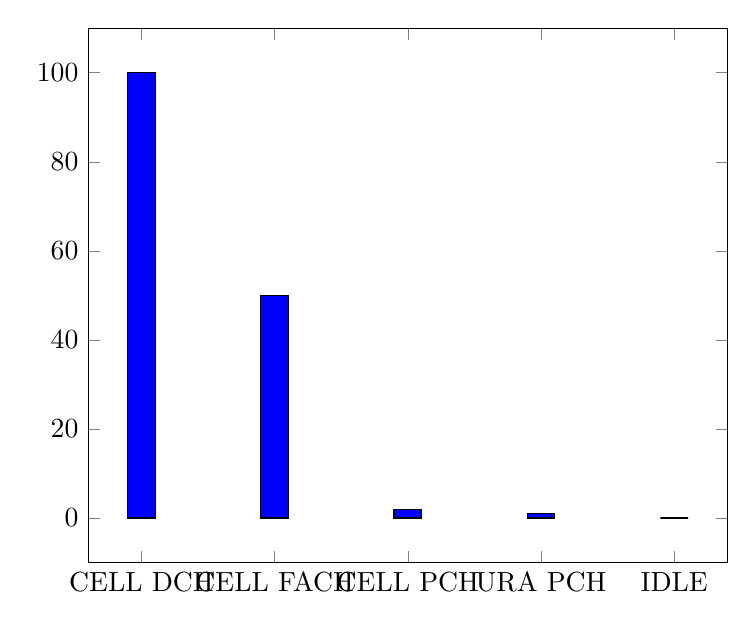
\begin{tikzpicture}
  \begin{axis}[
      width=0.80\textwidth,
      symbolic x coords={CELL DCH, CELL FACH, CELL PCH, URA PCH, IDLE},
      xtick=data
    ]
    \addplot[ybar,fill=blue] coordinates {
        (CELL DCH,   100)
        (CELL FACH,  50)
        (CELL PCH,   2)
        (URA PCH,    1)
        (IDLE,       0)
    };
  \end{axis}
  \label{graph:rrcPower}
\end{tikzpicture}

The graph above utilises ``theoretical'' values, however the percentages of 
these values are deemed to be correct. 

CELL DCH uses as much power as it can get, so in this example this is set to 
100\%. Devices that are in the CELL FACH state will only use around 50\% of the
power that the CELL DCH state would use, and CELL PCH would only use around 
2\%. URA PCH (if supported) would use 1\% of the CELL DCH state with IDLE 
utilising 0\% \citep{umtsworld}.

The RRC State selection is made at a mobile operator level. This means that one 
operator may choose to use all five states, where by another operator may only 
choose to use three. The different configurations and states leads to 
differences in energy consumption \citep{umtsworld}.

Unlike the previous terms, the RRC state will stay fixed throughout the 
duration of some activity (whether that be a call or data transfer). This 
project refers to the RRC state as the Start RRC state.